\chapter{जलना: आग को क्या चाहिए}\label{ch:g4:what-a-fire-needs}

शाम ढले \omterm{def:g4:what-a-fire-needs:burning}{जलता} अलाव। उसके लिए सूखी लकड़ी चाहिए थी, उसे सुलगाने के लिए
एक तीली, और उसमें से बहती \omterm{def:g4:air-a-mixture-of-gases:air}{हवा} उसे तेज़ बनाए रखती है। एक घंटे बाद लट्ठे
सिकुड़कर दहकते अंगारे और सफ़ेद राख बन गए हैं, और धूसर धुआँ उड़कर आकाश
में चला गया है। लकड़ी कहाँ गई? आग को क्या चाहिए, और वह पीछे क्या
छोड़ती है?

\begin{recall}
\omterm{def:g4:air-a-mixture-of-gases:air}{वायु} गैसों का एक मिश्रण है: लगभग चार-पाँचवाँ भाग नाइट्रोजन और पाँचवाँ
भाग ऑक्सीजन, थोड़ी-सी आर्गन और कार्बन डाइऑक्साइड के साथ। लौ अपने आस-पास
की \omterm{def:g4:air-a-mixture-of-gases:air}{वायु} से ऑक्सीजन लेती है; मर्तबान के नीचे रखी मोमबत्ती तब बुझ जाती है
जब बहुत कम ऑक्सीजन बचती है (\cref{ch:g4:air-a-mixture-of-gases})।
\end{recall}

\begin{omfigure}
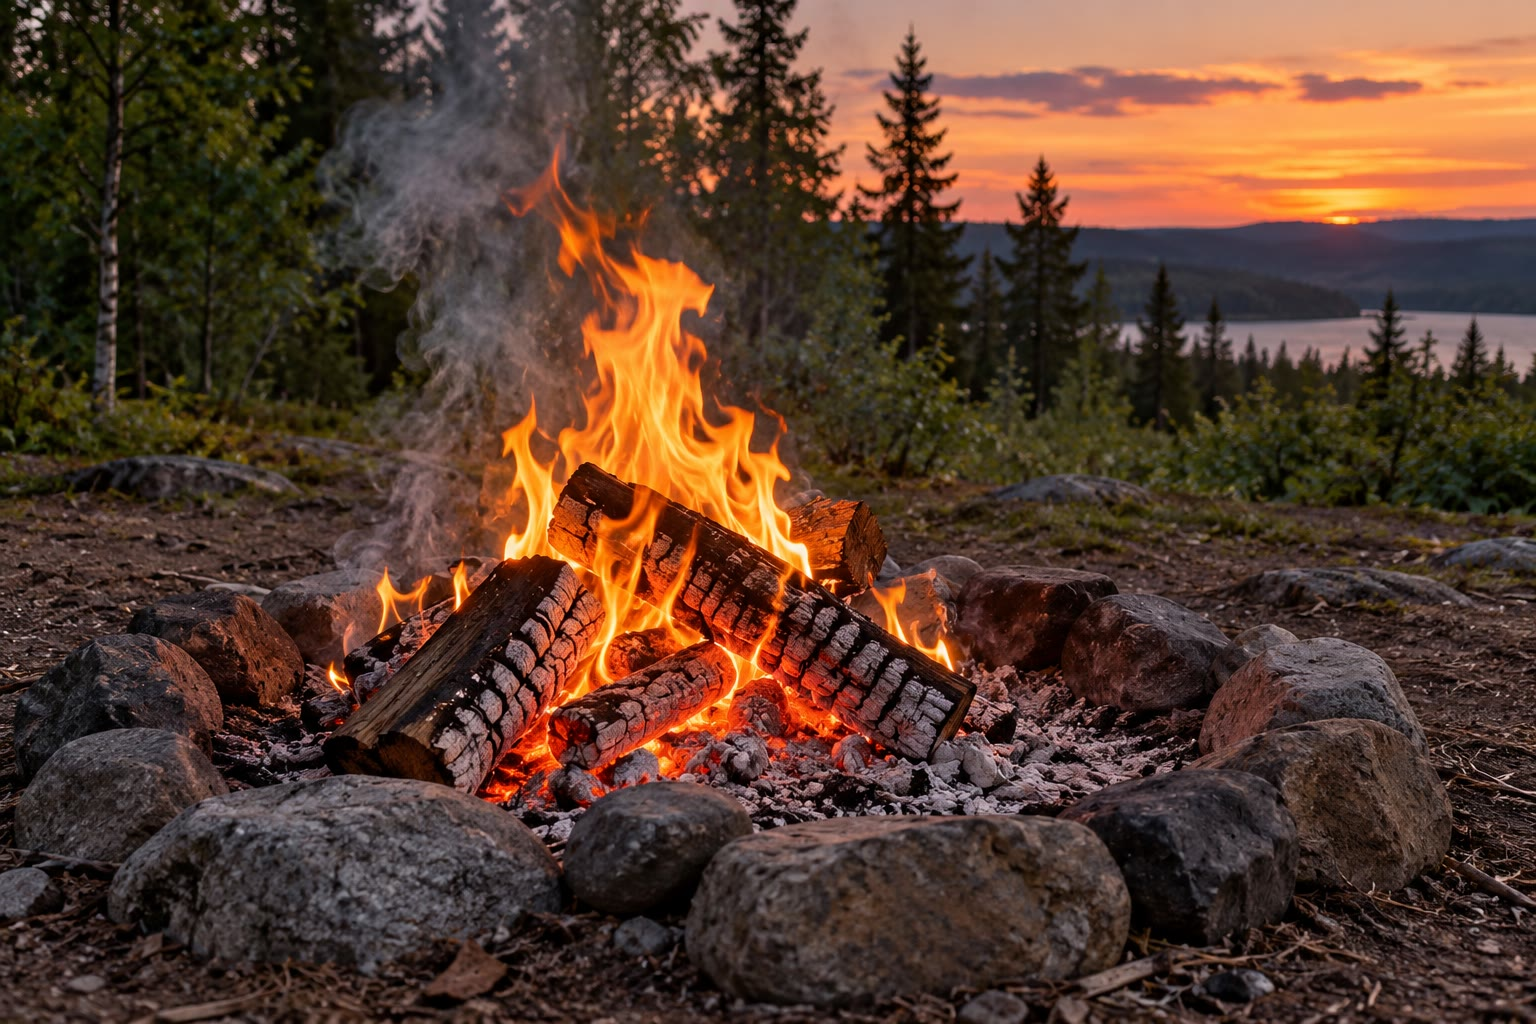
\includegraphics[width=0.6\linewidth]{images/book1/ai/g4-campfire.jpg}

{\small अलाव: लकड़ी, \omterm{def:g4:air-a-mixture-of-gases:air}{वायु} और एक तीली --- और बाद में राख और
धुआँ।}
\end{omfigure}

\section{ईंधन}

\begin{definition}[ईंधन]\label{def:g4:what-a-fire-needs:fuel}
\emph{ईंधन}\index{ईंधन} वह सामग्री है जो जलकर ऊष्मा और प्रकाश दे सकती
है: लकड़ी, कागज़, कोयला, मोमबत्ती का मोम, चूल्हे की गैस, पेट्रोल,
तापन तेल।
\end{definition}

\begin{example}[ठोस, द्रव और गैसीय ईंधन]\label{ex:g4:what-a-fire-needs:fuels}
लकड़ी, कागज़, कोयला और मोमबत्ती का मोम ठोस \omterm{def:g4:what-a-fire-needs:fuel}{ईंधन} हैं। पेट्रोल और तापन तेल
द्रव \omterm{def:g4:what-a-fire-needs:fuel}{ईंधन} हैं। रसोई के चूल्हे की गैस और लाइटर की गैस गैसीय
\omterm{def:g4:what-a-fire-needs:fuel}{ईंधन} हैं।
\end{example}

\begin{remark}[हर चीज़ नहीं जलती]\label{rem:g4:what-a-fire-needs:not}
पत्थर, रेत, काँच और पानी नहीं \omterm{def:g4:what-a-fire-needs:burning}{जलते}: वे \omterm{def:g4:what-a-fire-needs:fuel}{ईंधन} नहीं हैं। इसीलिए अँगीठी
पत्थर या ईंट की बनाई जाती है, और इसीलिए आग बुझाने के लिए रेत और पानी
का उपयोग होता है।
\end{remark}

\section{अग्नि त्रिभुज}

\begin{definition}[अग्नि त्रिभुज]\label{def:g4:what-a-fire-needs:fire-triangle}
आग को एक ही समय पर तीन चीज़ें चाहिए: \omterm{def:g4:what-a-fire-needs:fuel}{ईंधन}, \omterm{def:g4:air-a-mixture-of-gases:air}{वायु} की ऑक्सीजन, और उसे
शुरू करने के लिए ऊष्मा। इन तीन चीज़ों को एक त्रिभुज की तीन भुजाओं के रूप
में बनाया जाता है: यह \emph{अग्नि त्रिभुज}\index{अग्नि त्रिभुज} है। अगर
एक भुजा न हो, तो आग नहीं \omterm{def:g4:what-a-fire-needs:burning}{जलती}।
\end{definition}

\begin{omfigure}
\begin{tikzpicture}[font=\small]
  \coordinate (A) at (0,0); \coordinate (B) at (5,0); \coordinate (C) at (2.5,4.1);
  \draw[line width=3pt, brown!70!black] (A) -- (B);
  \draw[line width=3pt, omDef] (B) -- (C);
  \draw[line width=3pt, red!75!black] (C) -- (A);
  \node[below=4pt, font=\small\bfseries, brown!60!black] at (2.5,0) {ईंधन};
  \node[right=4pt, font=\small\bfseries, omDef] at (3.75,2.05) {ऑक्सीजन (वायु से)};
  \node[left=4pt, font=\small\bfseries, red!75!black] at (1.25,2.05) {ऊष्मा (शुरू करने को)};
  % a flame in the middle
  \fill[orange!80] (2.5,0.55) .. controls (1.95,1.15) and (2.35,1.75) .. (2.55,2.3)
    .. controls (2.75,1.75) and (3.05,1.15) .. (2.5,0.55);
  \fill[yellow!80] (2.5,0.7) .. controls (2.25,1.05) and (2.4,1.35) .. (2.52,1.65)
    .. controls (2.62,1.35) and (2.75,1.05) .. (2.5,0.7);
\end{tikzpicture}

{\small \omterm{def:g4:what-a-fire-needs:fire-triangle}{अग्नि त्रिभुज}: \omterm{def:g4:what-a-fire-needs:fuel}{ईंधन}, ऑक्सीजन और ऊष्मा, तीनों एक साथ।}
\end{omfigure}

\begin{example}[तीली जलाना]\label{ex:g4:what-a-fire-needs:match}
तीली के सिरे को उसकी डिबिया के किनारे पर रगड़ा जाता है। रगड़ उसे इतना
गरम कर देती है कि वह \omterm{def:g4:what-a-fire-needs:burning}{जलने} लगता है: यह त्रिभुज की ऊष्मा वाली भुजा है।
तीली की लकड़ी \omterm{def:g4:what-a-fire-needs:fuel}{ईंधन} है, और \omterm{def:g4:air-a-mixture-of-gases:air}{वायु} ऑक्सीजन लाती है।
\end{example}

\begin{example}[अंगारों पर फूँकना]\label{ex:g4:what-a-fire-needs:embers}
लगभग बुझते-से लगने वाले दहकते अंगारे फूँक मारने पर फिर से भभक उठते हैं:
फूँकने से अभी भी गरम \omterm{def:g4:what-a-fire-needs:fuel}{ईंधन} तक ज़्यादा \omterm{def:g4:air-a-mixture-of-gases:air}{वायु}, और इसलिए ज़्यादा ऑक्सीजन,
पहुँचती है।
\end{example}

\section{जलने से नए पदार्थ बनते हैं}

\begin{definition}[जलना और दहन]\label{def:g4:what-a-fire-needs:burning}
\emph{जलना}\index{जलना} वह है जो तब होता है जब कोई \omterm{def:g4:what-a-fire-needs:fuel}{ईंधन} \omterm{def:g4:air-a-mixture-of-gases:air}{वायु} से ऑक्सीजन
लेकर ऊष्मा और प्रकाश देता है। रसायनज्ञ जलने को
\emph{दहन}\index{दहन} कहते हैं। दहन के दौरान \omterm{def:g4:what-a-fire-needs:fuel}{ईंधन} और
ऑक्सीजन की खपत होती है, और नए पदार्थ प्रकट होते हैं: धुआँ, राख, कार्बन
डाइऑक्साइड और जलवाष्प।
\end{definition}

\begin{proposition}[जलने को उलटा नहीं किया जा सकता]\label{prop:g4:what-a-fire-needs:new}
आग की राख और धुआँ वापस लकड़ी नहीं बनते, हम कितना भी इंतज़ार करें।
\omterm{def:g4:what-a-fire-needs:burning}{जलने} से ऐसे नए पदार्थ बनते हैं जो पहले नहीं थे; \omterm{def:g4:what-a-fire-needs:fuel}{ईंधन} हमेशा के लिए
चला जाता है।
\end{proposition}

\begin{inthelab}[मोमबत्ती के ऊपर ठंडा गिलास]
शिक्षक एक ठंडे, सूखे काँच के बीकर को एक पल के लिए मोमबत्ती की लौ के ऊपर
उलटा पकड़ते हैं। गिलास का भीतरी भाग पानी की नन्ही बूँदों से धुँधला हो जाता
है: \omterm{def:g4:what-a-fire-needs:burning}{जलती} मोमबत्ती से बनी जलवाष्प ठंडे काँच पर फिर से द्रव बन गई है। \omterm{def:g4:what-a-fire-needs:burning}{जलती}
मोमबत्ती पानी बनाती है, और कार्बन डाइऑक्साइड भी, जिसे आगे के एक अध्याय
में आने वाले परीक्षण से पहचाना जा सकता है।
\end{inthelab}

\begin{omfigure}
\begin{tikzpicture}[font=\small, scale=1.3]
  % candle
  \fill[white, draw=black!50] (-0.25,0) rectangle (0.25,1.2);
  \draw[black!70] (0,1.2) -- (0,1.33);
  \fill[orange!85] (0,1.3) .. controls (-0.16,1.5) and (-0.06,1.75) .. (0,1.95)
    .. controls (0.06,1.75) and (0.16,1.5) .. (0,1.3);
  \fill[yellow!85] (0,1.36) .. controls (-0.08,1.5) and (-0.03,1.62) .. (0,1.72)
    .. controls (0.03,1.62) and (0.08,1.5) .. (0,1.36);
  % upturned cold beaker above
  \pic[transform shape, rotate=180] at (0,4.3) {beaker={0}{white}};
  \foreach \x/\y in {-0.6/3.9,-0.45/4.1,-0.2/3.95,0.1/4.15,0.35/3.9,0.6/4.05,
                     -0.7/3.5,0.7/3.4,-0.72/3.0,0.72/2.9}
    \fill[omDef!55] (\x,\y) circle (0.035);
  \draw[<-, omProp, thick] (0.68,3.95) -- (2.0,4.2) node[right, text=black]
    {पानी की बूँदें};
  \draw[<-, omProp, thick] (0.85,3.2) -- (2.0,3.3) node[right, text=black]
    {ठंडा गिलास, उलटा};
  \draw[<-, omProp, thick] (0.15,1.7) -- (2.0,1.9) node[right, text=black]
    {लौ: जलता हुआ मोम};
  \draw[<-, omProp, thick] (0.3,0.6) -- (2.0,0.7) node[right, text=black]
    {मोमबत्ती का मोम: ईंधन};
\end{tikzpicture}

{\small मोमबत्ती के ऊपर पकड़ा गया ठंडा गिलास धुँधला हो जाता है: \omterm{def:g4:what-a-fire-needs:burning}{जलता} मोम
जलवाष्प बनाता है।}
\end{omfigure}

\begin{example}[लट्ठा क्या बन जाता है]\label{ex:g4:what-a-fire-needs:log}
कुछ किलोग्राम का लट्ठा जलकर राख की एक छोटी-सी ढेरी रह जाता है। ज़्यादातर
लकड़ी ग़ायब नहीं हुई: \omterm{def:g4:air-a-mixture-of-gases:air}{वायु} की ऑक्सीजन के साथ मिलकर वह धुआँ, कार्बन
डाइऑक्साइड और जलवाष्प बन गई है, जो गैसें हैं और उड़कर आकाश में
चली जाती हैं।
\end{example}

\section{आग बुझाना}

\begin{method}[आग बुझाना: एक भुजा हटा दो]\label{met:g4:what-a-fire-needs:out}
आग बुझाने के लिए \omterm{def:g4:what-a-fire-needs:fire-triangle}{अग्नि त्रिभुज} की एक भुजा हटा दो:
\begin{itemize}
  \item \textbf{ऑक्सीजन हटाओ}: आग को अग्निरोधी कंबल, ढक्कन या रेत से
        ढक दो, ताकि \omterm{def:g4:air-a-mixture-of-gases:air}{वायु} उस तक न पहुँच सके;
  \item \textbf{ऊष्मा हटाओ}: \omterm{def:g4:what-a-fire-needs:burning}{जलती} लकड़ी या कागज़ पर पानी डालो, जो उसे
        इतना ठंडा कर देता है कि वह जल न सके;
  \item \textbf{\omterm{def:g4:what-a-fire-needs:fuel}{ईंधन} हटाओ}: गैस का नल बंद कर दो, या जंगल की आग के आस-पास
        के सूखे पौधे साफ़ कर दो।
\end{itemize}
\end{method}

\begin{omfigure}
\begin{tikzpicture}[font=\small, scale=0.7]
  \foreach \k/\lab/\side in {0/{कंबल: ऑक्सीजन नहीं}/1, 1/{पानी: ऊष्मा नहीं}/2,
                              2/{गैस बंद: ईंधन नहीं}/0} {
    \begin{scope}[xshift=\k*6.2cm]
      \coordinate (A) at (0,0); \coordinate (B) at (4,0); \coordinate (C) at (2,3.3);
      \pgfmathsetmacro\oa{\side==0 ? 0.2 : 1}
      \pgfmathsetmacro\ob{\side==1 ? 0.2 : 1}
      \pgfmathsetmacro\oc{\side==2 ? 0.2 : 1}
      \draw[line width=2.5pt, brown!70!black, opacity=\oa] (A) -- (B);
      \draw[line width=2.5pt, omDef, opacity=\ob] (B) -- (C);
      \draw[line width=2.5pt, red!75!black, opacity=\oc] (C) -- (A);
      \ifnum\side=0 \draw[line width=1.4pt, black] (1.6,-0.4) -- (2.4,0.4) (1.6,0.4) -- (2.4,-0.4);\fi
      \ifnum\side=1 \draw[line width=1.4pt, black] (2.6,1.25) -- (3.4,2.05) (2.6,2.05) -- (3.4,1.25);\fi
      \ifnum\side=2 \draw[line width=1.4pt, black] (0.6,1.25) -- (1.4,2.05) (0.6,2.05) -- (1.4,1.25);\fi
      \node[align=center, anchor=north] at (2,-0.6) {\lab};
    \end{scope}
  }
\end{tikzpicture}

{\small आग बुझाने के तीन तरीके, हर एक त्रिभुज की एक भुजा हटाता है
(काटी गई): ऑक्सीजन, ऊष्मा या \omterm{def:g4:what-a-fire-needs:fuel}{ईंधन}।}
\end{omfigure}

\begin{omfigure}
\begin{minipage}[t]{0.48\linewidth}\centering
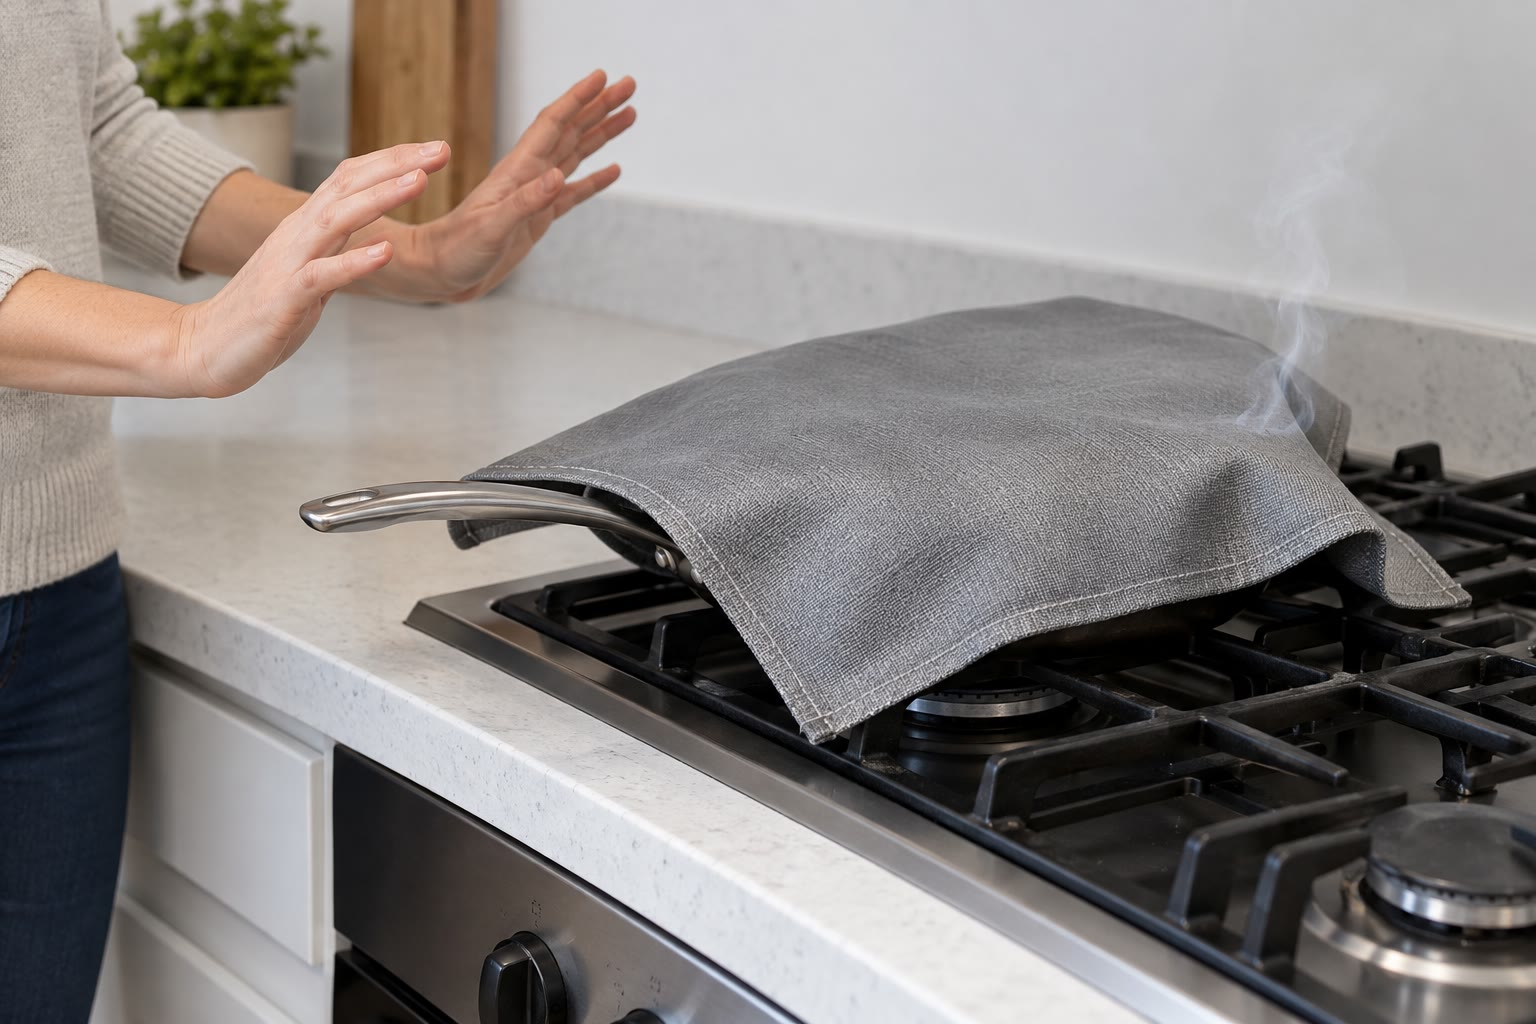
\includegraphics[width=\linewidth,height=4.6cm,keepaspectratio]{images/book1/ai/g4-fire-blanket.jpg}

{\small कड़ाही पर अग्निरोधी कंबल: \omterm{def:g4:air-a-mixture-of-gases:air}{वायु} अब आग तक नहीं पहुँच
सकती।}
\end{minipage}\hfill
\begin{minipage}[t]{0.48\linewidth}\centering
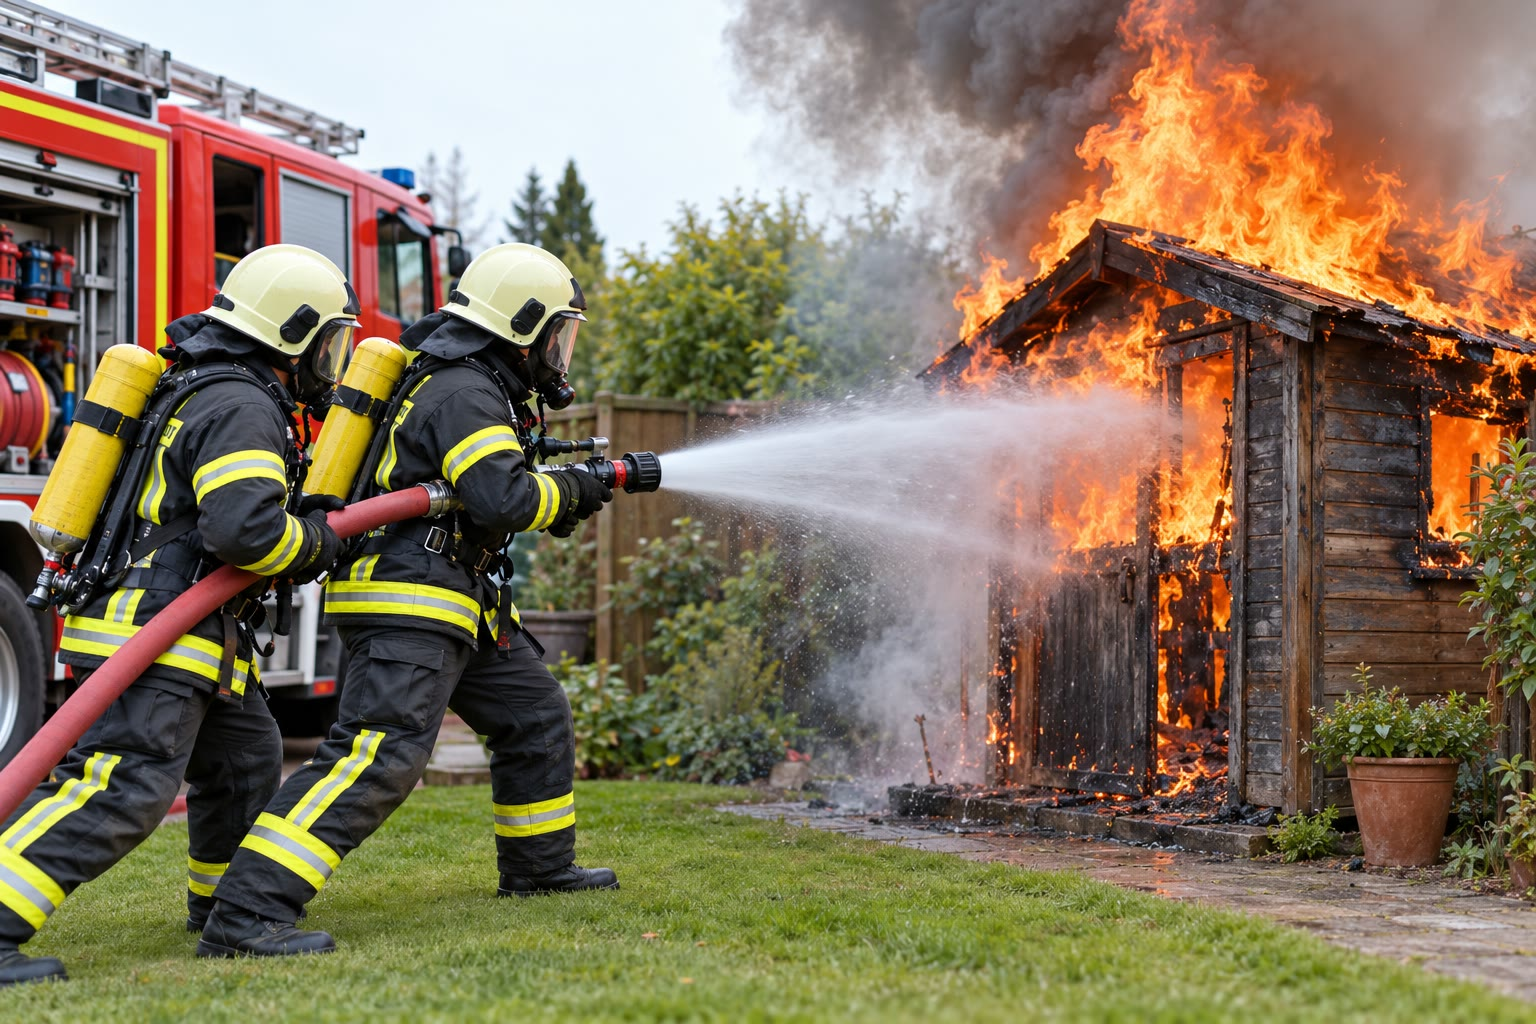
\includegraphics[width=\linewidth,height=4.6cm,keepaspectratio]{images/book1/ai/g4-firefighters.jpg}

{\small अग्निशमन कर्मी \omterm{def:g4:what-a-fire-needs:burning}{जलते} हुए छप्पर को ठंडा करने के लिए पानी की बौछार करते हैं।}
\end{minipage}
\end{omfigure}

\section{आग से सुरक्षा}

\begin{remark}[जलते तेल की कड़ाही पर कभी पानी नहीं]\label{rem:g4:what-a-fire-needs:oil}
अगर कड़ाही के तेल में आग लग जाए, तो उस पर कोई पानी न फेंके: पानी तेल के
नीचे तुरंत उबल जाता है और \omterm{def:g4:what-a-fire-needs:burning}{जलते} तेल को कड़ाही से बाहर उछाल देता है। गैस या
हॉटप्लेट बंद की जाती है और कड़ाही को ढक्कन या अग्निरोधी कंबल से ढका जाता
है --- यह काम कोई बड़ा व्यक्ति करता है।
\end{remark}

\begin{safety}{\ghs{GHS02}\ghs{GHS04}}
% ledger: ghs:butane
लाइटर या कैंपिंग कारतूस की गैस ब्यूटेन है। उसका लौ वाला
चित्रसंकेत (GHS02) बताता है: अत्यंत ज्वलनशील, लौ और चिंगारियों से दूर
रखें। गैस सिलिंडर वाला चित्रसंकेत (GHS04) बताता है: दाब में रखी
गई गैस।
\end{safety}

\begin{proposition}[आग लगने पर क्या करें]\label{prop:g4:what-a-fire-needs:safety}
आग का पहला ख़तरा धुआँ है: वह गरम होता है, बाहर निकलने का रास्ता छिपा
देता है और साँस में लेने पर ज़हरीला होता है। छत पर लगा धुआँ-अलार्म
धुआँ पहुँचते ही ज़ोर से बीप करता है। अगर आग लगे: बाहर निकलो, धुएँ के
नीचे झुककर चलो, पीछे के दरवाज़े बंद करते जाओ, और बाहर से अग्निशमन दल को
फ़ोन करो। कभी वापस अंदर मत जाओ।
\end{proposition}

\begin{omfigure}
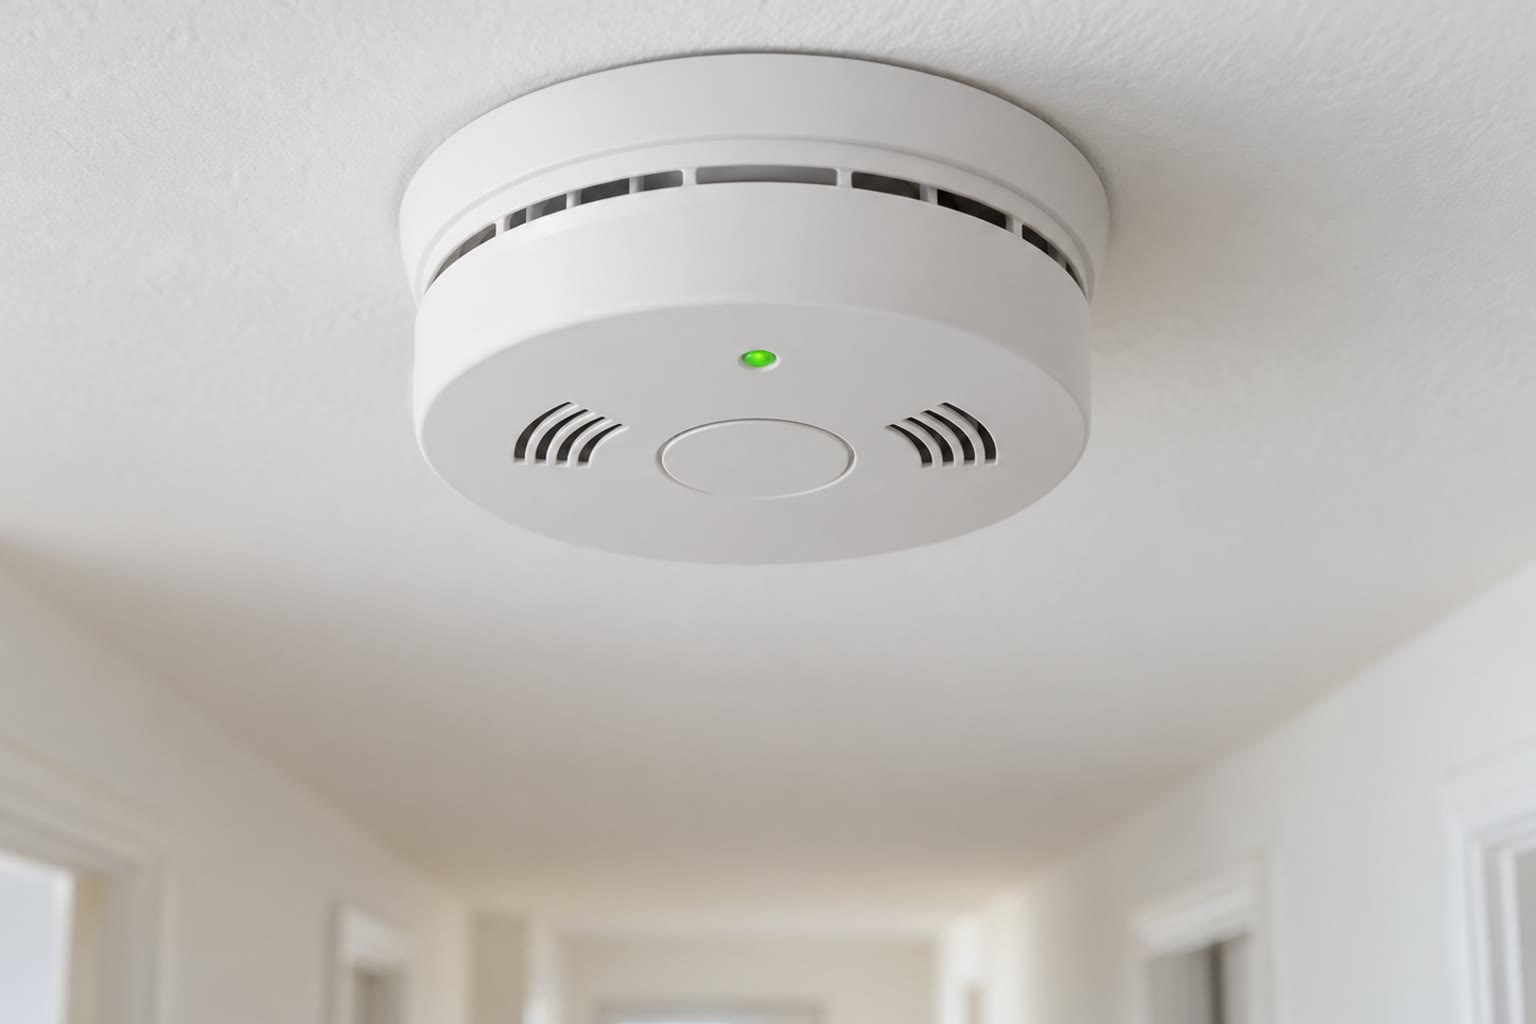
\includegraphics[width=0.42\linewidth]{images/book1/ai/g4-smoke-alarm.jpg}

{\small धुआँ-अलार्म: धुआँ पहुँचते ही यह बज उठता है।}
\end{omfigure}

\section{अभ्यास}

\begin{exercise}[$\star$]\label{exo:g4:what-a-fire-needs:1}
\omterm{def:g4:what-a-fire-needs:fire-triangle}{अग्नि त्रिभुज} की तीनों भुजाओं के नाम बताओ।
\end{exercise}

\begin{exercise}[$\star$]\label{exo:g4:what-a-fire-needs:2}
इनमें से कौन-से \omterm{def:g4:what-a-fire-needs:fuel}{ईंधन} हैं: लकड़ी, रेत, मोमबत्ती का मोम, काँच, पेट्रोल, पानी,
कागज़?
\end{exercise}

\begin{exercise}[$\star$]\label{exo:g4:what-a-fire-needs:3}
एक छोटी-सी आग पर अग्निरोधी कंबल डाला जाता है। वह \omterm{def:g4:what-a-fire-needs:fire-triangle}{अग्नि त्रिभुज} की कौन-सी
भुजा हटाता है?
\end{exercise}

\begin{exercise}[$\star$]\label{exo:g4:what-a-fire-needs:4}
अग्निशमन कर्मी \omterm{def:g4:what-a-fire-needs:burning}{जलते} छप्पर पर पानी की बौछार करते हैं। पानी \omterm{def:g4:what-a-fire-needs:fire-triangle}{अग्नि त्रिभुज} की
कौन-सी भुजा हटाता है?
\end{exercise}

\begin{exercise}[$\star$]\label{exo:g4:what-a-fire-needs:5}
लकड़ी \omterm{def:g4:what-a-fire-needs:burning}{जलने} पर बनने वाले तीन नए पदार्थों के नाम बताओ।
\end{exercise}

\begin{exercise}[$\star$]\label{exo:g4:what-a-fire-needs:6}
दहकते अंगारों पर फूँकने से वे फिर क्यों भभक उठते हैं?
\end{exercise}

\begin{exercise}[$\star$]\label{exo:g4:what-a-fire-needs:7}
मोमबत्ती के ऊपर पकड़ा गया ठंडा गिलास धुँधला हो जाता है। मोमबत्ती ने कौन-सा
नया पदार्थ बनाया है?
\end{exercise}

\begin{exercise}[$\star$]\label{exo:g4:what-a-fire-needs:8}
अगर धुआँ-अलार्म बजे और तुम्हें धुआँ दिखे, तो सबसे पहले क्या करना चाहिए?
\end{exercise}

\begin{exercise}[$\star$]\label{exo:g4:what-a-fire-needs:9}
तीन छोटे त्रिभुजों वाला चित्र देखो। गैस बंद करने पर कौन-सी भुजा काटी
जाती है?
\end{exercise}

\begin{exercise}[$\star\star$]\label{exo:g4:what-a-fire-needs:10}
जंगल की आग को रोकने के लिए अग्निशमन कर्मी कभी-कभी उसके आगे पेड़ों की एक
चौड़ी पट्टी काट देते हैं। वे \omterm{def:g4:what-a-fire-needs:fire-triangle}{अग्नि त्रिभुज} की कौन-सी भुजा हटा
रहे हैं?
\end{exercise}

\begin{exercise}[$\star\star$]\label{exo:g4:what-a-fire-needs:11}
लट्ठा अपनी राख से बहुत भारी होता है। क्या लट्ठे का कुछ भाग ग़ायब हो गया?
समझाओ कि वह कहाँ गया।
\end{exercise}
